% -*- TeX-master: "../dipole_ilya_paper.tex" -*-
\section{Fabrication}

\begin{figure}[h]
  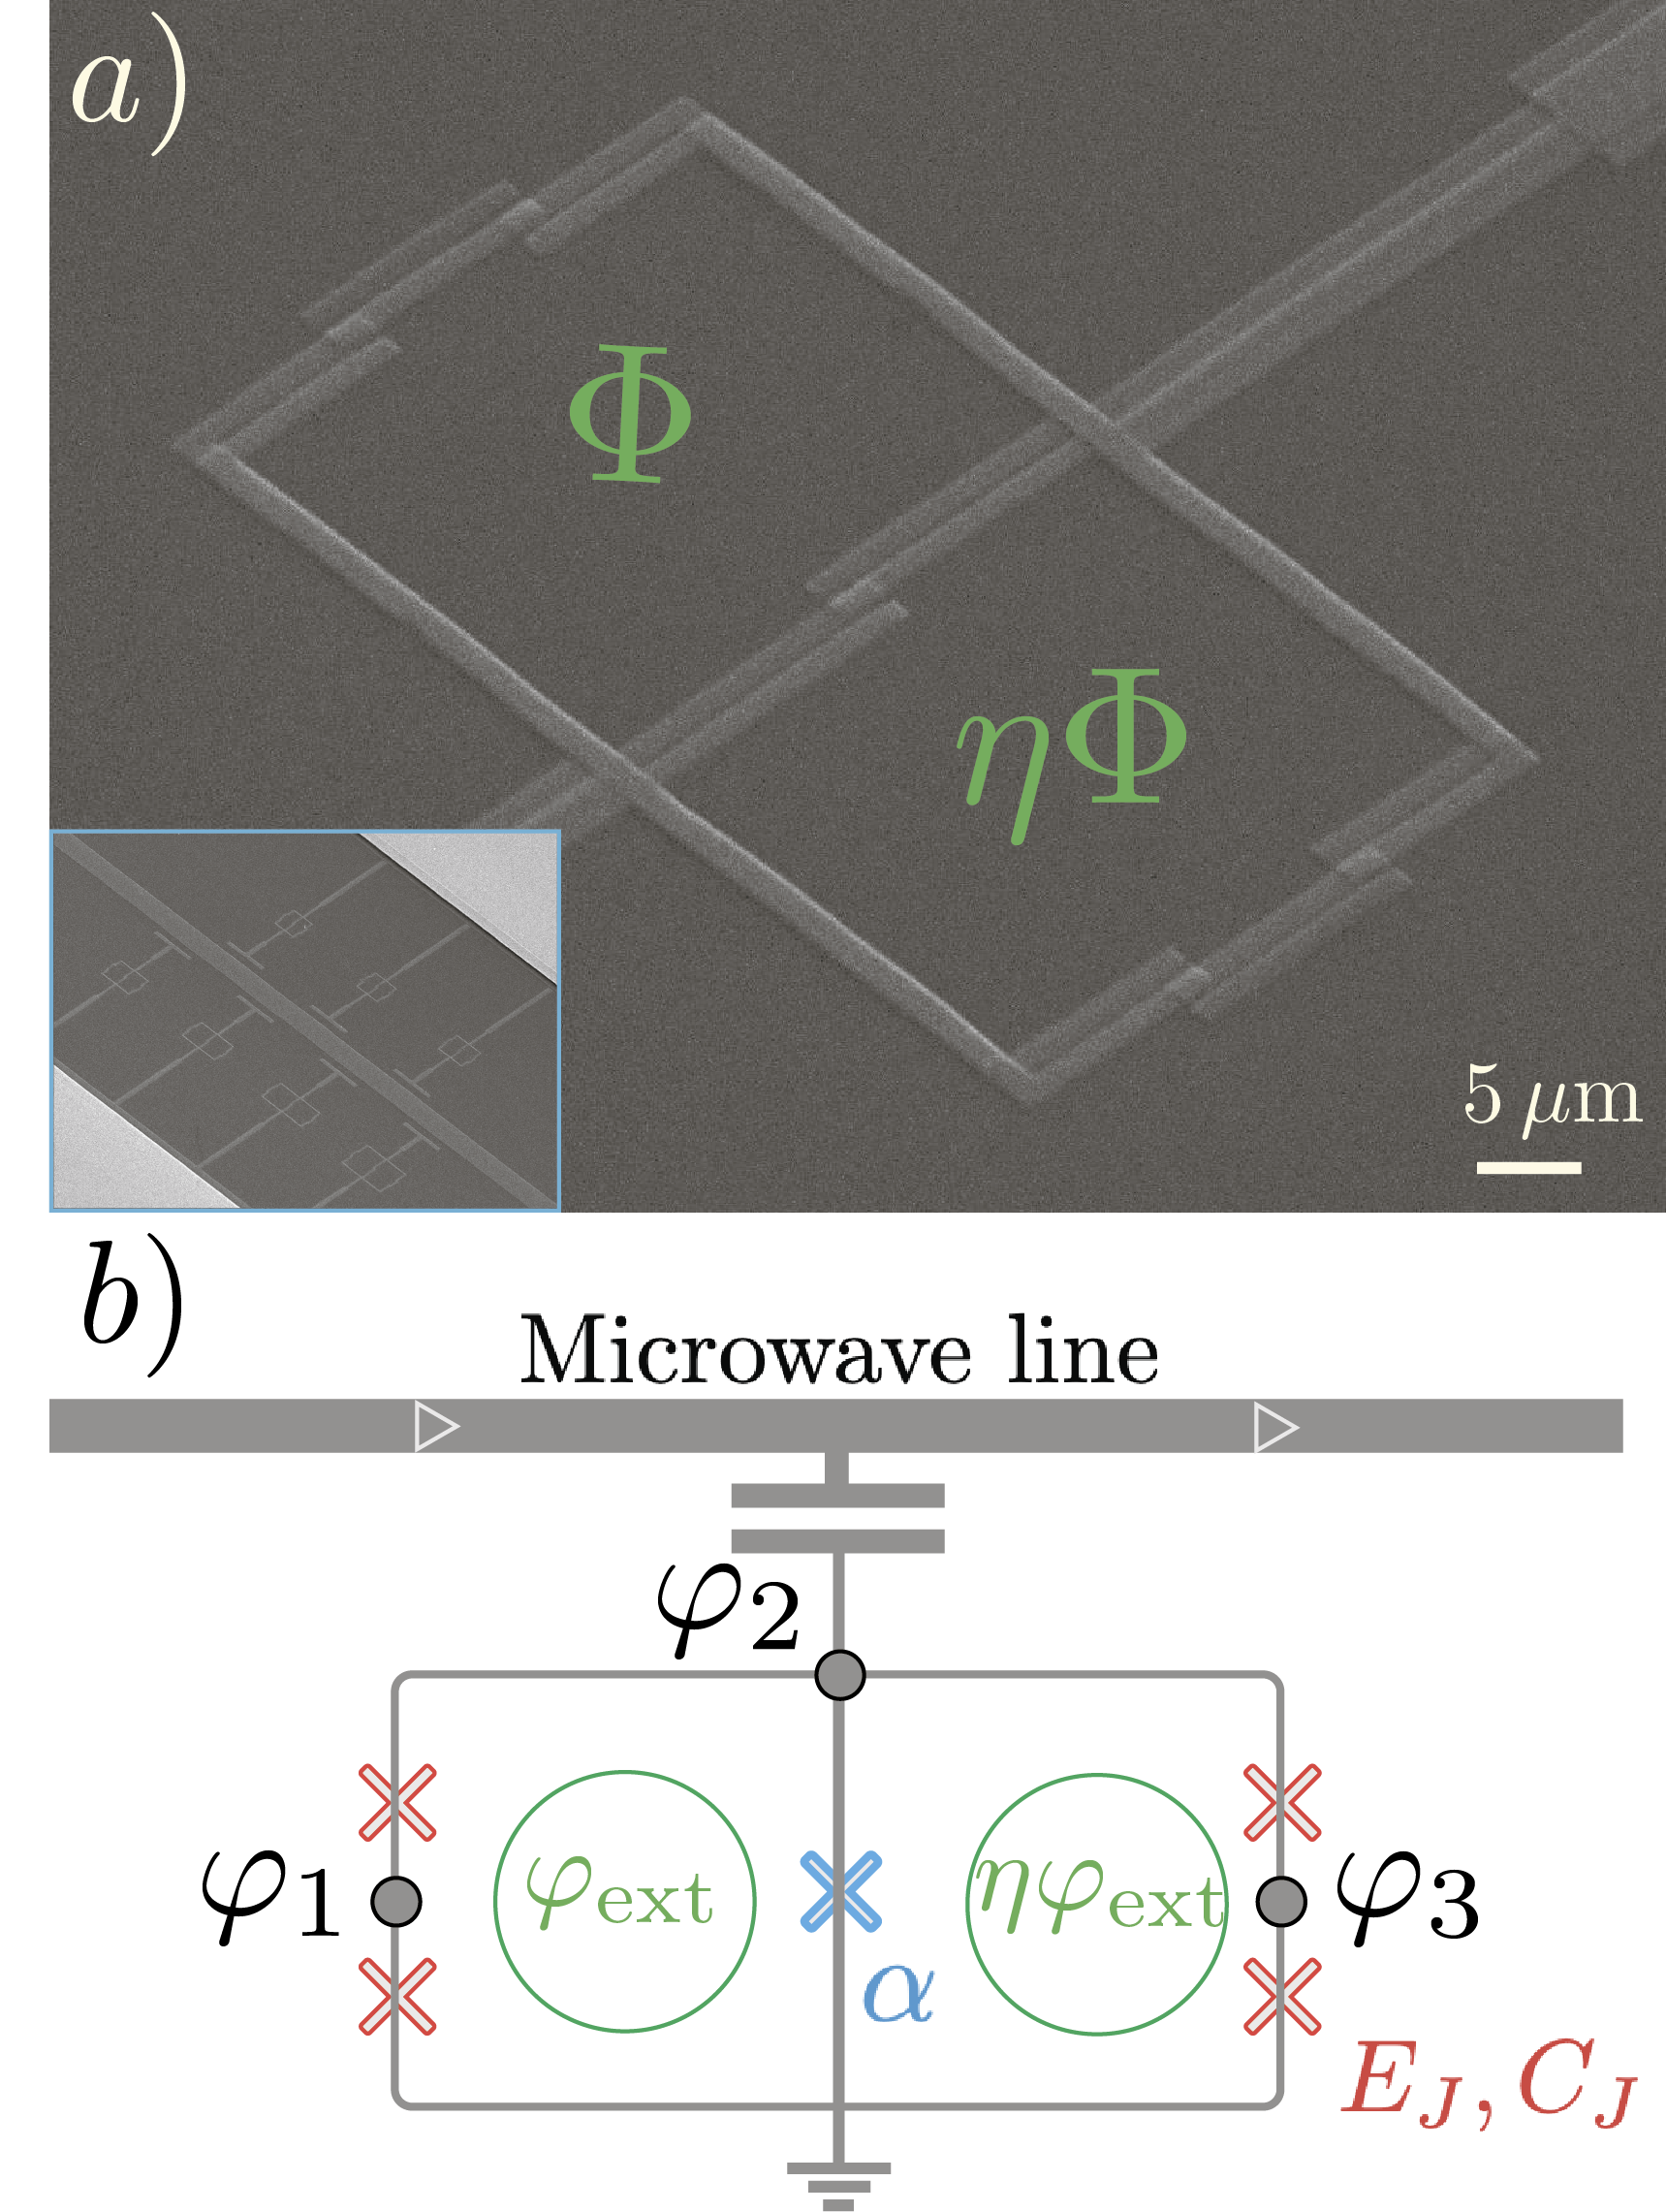
\includegraphics[height=10.5cm]{figure1_v2}
  \caption{\small Geometry of a twin qubit: a) Scanning electron microscope (SEM) image of the qubit flux biases $ \Phi $,
    $ \eta\Phi $ applied to it's superconducting loops. The qubit has a macroscopic size $ \sim 20\,\mu $m coupled to a microwave line with
    T-shaped capacitors (inset); b) The central junction has an energy of $ \alpha E_{J}$ capacitance $\alpha C$ relative to the outside
    JJs.}
    \label{fig:setup}
  % \caption{\small{Scanning electron microscope image of the dipole
  % qubits capacitively coupled to the tranmisssion line. A common
  % flux $ \Phi $ is applied to each loop with an external magnetic
  % field. This magnetic field effects the phases induced across the
  % junction$ \varphi_i$ .} Phases will arange is such a way, so that
  % potential energy is minimised}
\end{figure}

%% Describe fabrication
\noindent The qubit is fabricated on undoped silicon. It is coupled to a coplanar transmission line, with an impedance of
$ Z_{0} \approxeq 50\,\Omega $, which passes through to an opening in the center of the chip. Twin qubits and T-shaped coupling capacitors are
fabricated simultaneously using the shadow evaporation technique \includeref{paper on shadow evaporation} of aluminum with
intermediate oxidation. These steps result in a 5-JJ structure of Fig.~\ref{fig:setup}. Measurements were performed in a 14\,mK
environment to suppress thermal activation. The micrwoave signals were delivered to the qubit via a single transmission line.

%% Explain how other new qubits have been fabricated with grooves and HF - this is down the line for this type of geometry

%%% Local Variables:
%%% mode: latex
%%% TeX-master: "../dipole_ilya_paper"
%%% End: